\documentclass[11pt,a4paper]{article}

\usepackage{amsmath}
\usepackage{amsfonts}
\usepackage{amssymb}
\usepackage{graphicx}
\graphicspath{{images/}}


\begin{document}

\newcommand{\N}{\mathbb{N}}
\newcommand{\R}{\mathbb{R}}
\newcommand{\Z}{\mathbb{Z}}
\newcommand{\e}{\varepsilon}
\newcommand{\bb}[1]{\boldsymbol{#1}}

\section{HB}

HB is an authentication protocols first introduced by Blum et al. \cite{10.1007/3-540-45682-1_4}, \cite{10.1007/3-540-48329-2_24} that relies on the hardness of the learning parity with noise problem (LPN) for security and is provably secure against passive attacks. Figure \ref{fig1} shows one iteration of the authentication of HB.

\begin{figure}[h]
	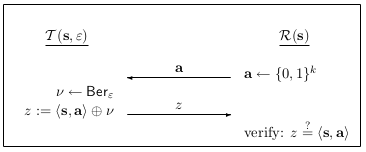
\includegraphics[width=8cm]{hb}
	\centering
	\caption{One iteration of the HB protocol}
	\label{fig1}
\end{figure}

A tag $\mathcal{T}$ and a reader $\mathcal{R}$ share a random secret key $\bb{s} \in \{0,1\}^k$. One iteration (all of which happen in parallel) of the authentication step consists of the following:
$\mathcal{R}$ sends a random challenge $\bb{a} \in \{0,1\}^k$ to $\mathcal{T}$ who in turn calculates $\bb{z}:= \langle \bb{s}, \bb{a} \rangle \oplus v$ with $v \leftarrow \text{Ber}_\e$.
This result is sent back to $\mathcal{R}$ who then calculates if the iteration is \textit{successful}, i.e. $\bb{z} = \langle \bb{s}, \bb{a} \rangle $. Notice that even iterations of an honest tag using the correct key $s$ can be unsuccessful with probability $\e$. The reader therefore accepts the authentication of the tag if the number of unsuccessful iterations is at most $\approx \e \cdot n$.

\section{HB+}

A modification of the HB protocol in order for it to be secure against an active adversary is the HB+ protocol by Juels and Weis \cite{juels2005authenticating} shown in Figure \ref{fig2}.

\begin{figure}[h]
	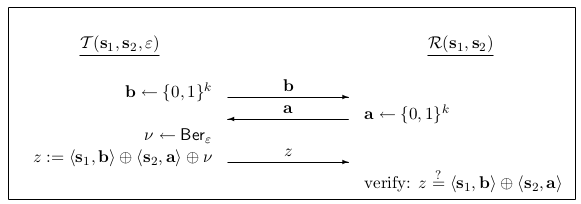
\includegraphics[width=11cm]{hbp}
	\centering
	\caption{One iteration of the HB+ protocol}
	\label{fig2}
\end{figure}

 $\mathcal{R}$ and $\mathcal{T}$ now share two secret keys $\bb{s_1}, \bb{s_2} \in \{0,1\}^k$. One iteration of the authentication step now looks as follows:
$\mathcal{T}$ first sends a random "blinding factor" $\bb{b} \in \{0,1\}^k$ to $\mathcal{R}$. The reader then, as for HB, sends a random challenge $\bb{a} \in \{0,1\}^k$ to $\mathcal{T}$ who in turn calculates $z:= \langle \bb{s_1}, \bb{b} \rangle \oplus \langle \bb{s_2}, \bb{a} \rangle \oplus v$ with $v \leftarrow \text{Ber}_\e$.
This result is sent back to $\mathcal{R}$ who then calculates if the iteration is \textit{successful}, i.e. $z = \langle \bb{s_1}, \bb{b} \rangle \oplus \langle \bb{s_2}, \bb{a} \rangle$. Again, even if $\mathcal{T}$ sends an honest $z$ using the correct keys $\bb{s_1}$, $s_2$ the iteration can be \textit{unsuccessful}. Therefore, up to $\approx e \cdot n$ \textit{unsuccessful} iterations are allowed fot the tag to still be accepted.

\section{AUTH, MAC1, MAC2}

The AUTH protocol shown in Figure \ref{fig3} was introduced by Kiltz et al. \cite{Kiltz2017} and represents a two-round authentication protocol secure against active attacks and man-in-the-middle attacks, even in a quantum setting. The security of this protocol relies on the \textit{subspace LPN problem} which is reducible to LPN.

\begin{figure}[h]
	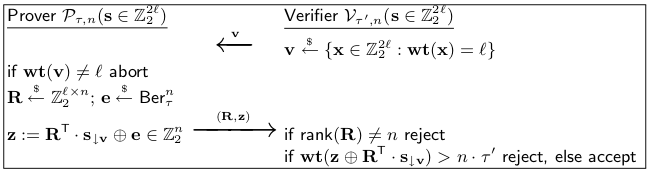
\includegraphics[width=11cm]{auth}
	\centering
	\caption{Two-round authentication protocol AUTH}
	\label{fig3}
\end{figure}

Whereas the random challenges $\bb{R} \in \Z_2^{l \times n}$ (each row of the matrix $\bb{R}^T$ corresponding to one challenge $a$ in HB) were computed by the Verifier $\mathcal{V}$ in HB, they are now computed by the Prover $\mathcal{P}$.
$\mathcal{V}$ instead sends a random vector $\bb{v} \in \Z_2^{2l}$ with Hamming weight $\text{wt}(\bb{v}) = l$ to select $l$ of the $2l$ key bits of $s$ to produce a key subset $\bb{s}_{\downarrow v}$ which is derived from $\bb{s}$ by deleting all bits $\bb{s}[i]$ where $\bb{v}[i] = 0$.
Then, $\bb{z} \in \Z_2^n$ is computed as $\bb{R}^T \cdot \bb{s}_{\downarrow v} \oplus \bb{e}$ and sent to $\mathcal{V}$ along with $\bb{R}$.
$\mathcal{V}$ rejects the authentication if either $\text{rank}(\bb{R}) \neq n$ or if the number of unsuccessful iterations denoted as $\text{wt}(\bb{z} \oplus \bb{R}^T \cdot \bb{s}_{\downarrow v})$ is greater than the threshold $n \cdot \tau'$ with $\tau' = 0.25 + \tau/2$.




\newpage
\addcontentsline{toc}{section}{\refname}
\bibliographystyle{alpha}
\bibliography{references}

\end{document}
